\section{Einleitung}
\label{sec:einleitung}

\subsection{Motivationen und Hintergr�nde}
\label{sec:einleitung:motivation}
Soll ein neu zu erstellendes Softwaresystem auf Basis vorhandener Komponenten erstellt werden, so stellt sich h�ufig die Frage nach der Perfomance des Gesamtsystems. Deren Beantwortung vor der Implementierung ist h�ufig Vorraussetzung zur Einhaltung einiger nichtfunktionaler Anforderungen wie zum Beispiel der mittlere Antwortzeit. Sind die Antwortzeiten der Dienste der einzelnen Komponenten h�ufig bekannt, so gilt es nun die Antwortzeit des Gesamtsystems mit einer bestimmten Konfiguration dieser Komponenten und ggf. Konnektoren zu ermitteln. Weiterhin ist h�ufig die Aufdeckung von 'Flaschenh�lsen' im System hilfreich, um durch eine gezielt andere Konfiguration der Komponenten die Performance zu erh�hen.
\par
Besteht das System ausschlie�lich aus linear zusammenh�ngenden Komponenten, deren Dienste der Reihe nach von einer ankommenden Anfrage durchlaufen werden, so gestaltet sich die Analyse des Systems recht einfach. Problemf�lle lassen sich anhand der Einzelzeiten identifizieren und die gesamte Antwortzeit kann durch Addition der Einzelzeiten relativ leicht ermittelt werden.\\
Beinhalteten die Komponenten innerhalb des Systems jedoch Verzweigungen, so m�ssen alle sich ergebenen Pfade einzeln berechnet und mit einer bestimmten Gewichtung gewertet werden.\\
Weiterhin ergibt es sich in Systemen h�ufig, das bestimmte Dienste einer Komponente von mehren Diensten des Gesamtsystems ben�tigt werden. Ein Beispiel hierf�r sind Dienste, die Daten aus einer Datenbank auslesen. Hierbei geht die Analyse des Systems �ber die Pfade hinaus. Es m�ssen nun die Antwortzeiten der Dienste der Komponenten dynamisch auf die Anzahl zu einem Zeitpunkt ankommender Anfragen angepasst werden.\\
�bersteigt die mathematisch exakte Analyse des Systems bereits hier die Grenzen des sinnvoll machbaren, so erscheint die exakte Berechnung bei der Verteilung der einzelnen Komponenten auf verschiedene Prozessoren als unm�glich.
\par
An dieser Stelle kann die Simulation ansetzen. Es werden nun nicht mehr die mathematisch exakten Gegebenheiten berechnet sondern anhand der Simulation eines Modells mit einer bestimmten Ungenauigkeit ermittelt. Weiterhin lassen sich bei der Simulation 'Flaschenh�lse' identifizieren, die bei der mathematischen Berechnung nur schwer zu ermitteln sind. Hierzu kann beispielsweise einfach das Zeitverhalten einer Anfrage Dienst f�r Dienst aufgezeichnet und hinterher ausgewertet werden. Bild \ref{pic:simul} zeigt schematisch eine solche Simulation.

\begin{figure}[ht]
\label{pic:simul}
\begin{center}
\fbox{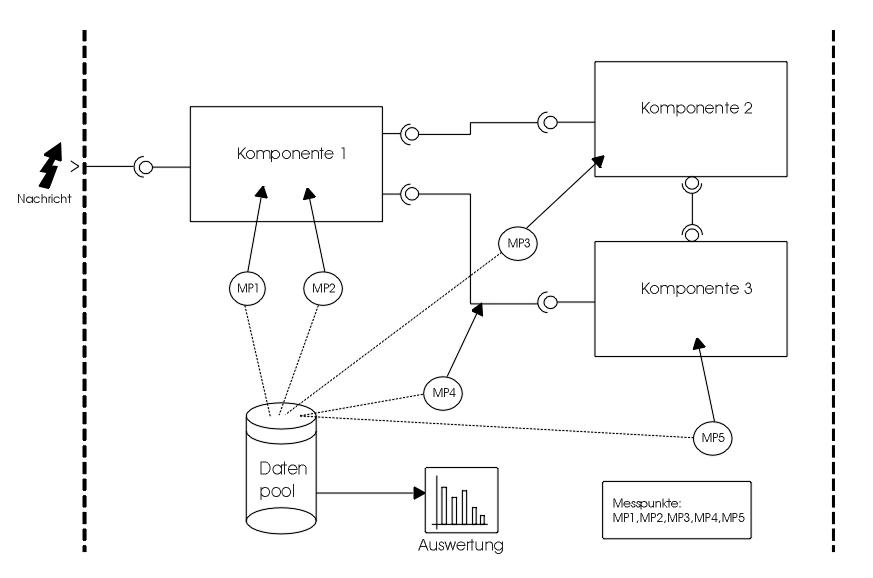
\includegraphics[width=13cm]{../res/simul.jpg}}
\caption{Schematische Darstellung der Simulation}
\end{center}
\end{figure}

\subsection{Ziele des Individuellen Projektes}
\label{sec:einleitung:ziele}
Ziel dieses Projektes ist die Erstellung einer Infrastruktur f�r die in Abschnitt \ref{sec:einleitung:motivation} erl�uterte Simulation in Form eines Frameworks. Bestandteil des Frameworks wird die Modulierung des Systems und der Komponenten, ein Modell zur Simulation von Anfragen an Dienste des Systems und die Auswertung der gesammelten Daten sein. Dies Bestandteile werden in einer Simulationmsumgebung gekapselt.
\par
Bei der Entwicklung wird verst�rkt darauf geachtet, dass Anwendungen das Frameworks sowohl statisch als auch dynamisch nutzen k�nnen. Dies bedeutet, dass das Framework zwei Modi zu Verf�gung stellt. Im ersten Fall wird es mit einer (z.B. durch eine XML-Datei) fest vorgegebenen Simulationsumgebung initialisiert und die Simulation gestartet. Der zweite dynamische Modus erlaubt den Aufbau und die Ver�nderung der Simulationsumgebung zur Laufzeit, was sich zur Entwicklung von grafischen Simulationsumgebungen eignet.
\par


\subsection{Aufbau dieser Ausarbeitung}
\label{sec:einleitung:aufbau}
